\section{Human Detection} \label{ch3}
The goal of the \textbf{human detection} problem is to detect and localize persons in an image regardless of their position, scale, pose, orientation and illumination.

\begin{figure}[h!]
		\centering
		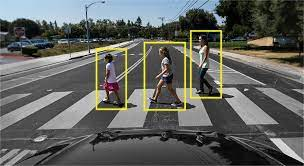
\includegraphics[scale = 0.7]{img/pedestrian recognition.jpeg}
        \caption{Pedestrian recognition problem}
\end{figure}

The main difficulties of this problem are:

\begin{itemize}
    \item The wide variety of articulated \textit{poses};
    \item Variable \textit{appearance and poses};
    \item Complex \textit{background};
    \item \textit{Occlusion};
\end{itemize}

\subsection{Research issues}
The main issues of \textit{pedestrian recognition} problem are very similar to the \textit{face detection}'s ones:

\begin{itemize}
    \item \textbf{Representation}, i.e. how to describe a typical person;
    \item \textbf{Scale}, i.e. how to deal with persons with different sizes;
    \item \textbf{Search strategy}, i.e. how to spot the persons;
    \item \textbf{Post-processing}, i.e. how to combine detection results.
\end{itemize}

\subsection{Method}
The usual method for solving the problem of \textit{pedestrian recognition} is given by the \textit{sliding window} approach, in particular by following these steps:

\begin{enumerate}
    \item \textbf{Inspect} every window of the image at all scales and locations;
    \item Given a window, extract a \textbf{feature vector}, i.e. a vector of numbers that describes the window's contents;
    \item \textbf{Classify} each feature vector and accept a window if the score is above a certain threshold;
    \item \textbf{Post-processing} phase in which the mess is cleaned-up.
\end{enumerate}

In the following sections we describe in detail each of the phase.

\subsubsection{Inspection phase}
In this phase, the \textbf{sliding window} scans the whole image at all scales and locations: usually, the window is 128 pixels tall and 64 pixels wide, as represented in Picture \ref{sliding_window}. This 2-to-1 aspect ratio is a rough compromise between the aspect ratio of a person viewed from the front and one viewed from the side with legs fully extended during a step.

\begin{figure}[h!]
		\centering
		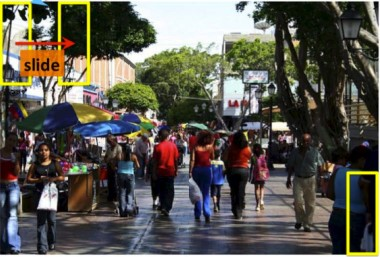
\includegraphics[scale = 1.5]{img/sliding window.jpg}
        \label{sliding_window}
        \caption{Sliding window}
\end{figure}

Moreover, in order for the \textit{pedestrian detector} to detect persons of very different scales in the same image, the window also scans a down-scaled version of the image, while the size of the window remains the same. This operation is repeated for many down-scaled version of the image, where the scale differences across the scans are small.

\subsubsection{Feature vector}
The second phase of the \textit{pedestrian recognition} solving method is given by the \textit{feature vector} creation. Since the method which is used for creating each feature vector is based on another family of methods, we first introduce the latter methods in order to better understand the former one.

\underline{Support Vector Machines (SVM)}
\\
One of the most important family of ML algorithm is represented by the \textbf{Support Vector Machines (SVM)}, which were introduced after the diffusion of the \textit{Backpropagation} algorithm, and which are very connected to \textit{Statistical Learning Theory}. \textit{SVM} deals with 
binary classification problems (with the assumption that the problem is linearly separable), and it belongs to the class of \textit{discriminative classifiers}, since its goal consists on learning the class boundary between the two classes $y$ starting from features $x$. More specifically, the goal of \textit{SVM} is to find, among all the possible class boundaries between the two classes, the one that is furthest from the two classes. If the distance between the closest points of two different classes is called \textbf{margin}, then \textit{SVM}'s goal is to separate the instances of the two classes with a boundary that \textbf{maximizes the margin}: intuitively, the farthest the boundary is from the points, the greater the confidence in the prediction is. Picture \ref{margin} provides a visual representation of the margin: the instances of the two classes that determine the margin, i.e. the red circled points, are called \textbf{support vectors}. In this sense, we can easily notice that decision boundary only depends on the support vectors, since they're the only points that determine the width of the margin. 

\begin{figure}[h!]
		\centering
		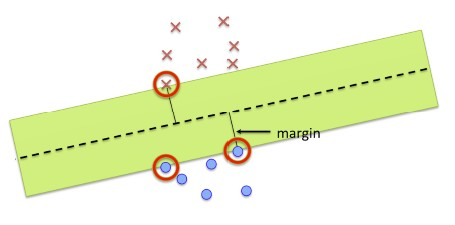
\includegraphics[scale = 1.5]{img/margin.jpg}
        \label{margin}
        \caption{Margin and support vectors}
\end{figure}

If we denote as $w^tx + b = 0$ (or, equivalently, as $c(w^tx + b) = 0$) the plane which separates the instances of the two classes, i.e. the decision boundary, then we can normalize the points of the dataset so that the \textit{positive} support vectors, i.e. the support vectors \textit{above} the decision boundary, lie on this plane:

$$
w^tx + b = +1
$$
, while the \textit{negative} support vectors on this one:

$$
w^tx + b = -1
$$

In this way, the distance between each support vector and the decision boundary is given by $\frac{1}{||w||}$, so the \textbf{equation of the margin} is $\frac{2}{||w||}$. A visual representation of these relationships is provided in Picture \ref{margin2}.

\begin{figure}[h!]
		\centering
		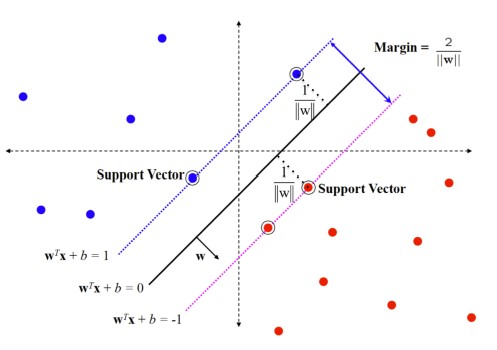
\includegraphics[scale = 1.7]{img/margin2.jpg}
        \label{margin2}
        \caption{Margin and support vectors}
\end{figure}

As we said before, the goal of \textit{SVM} is to maximize the margin, so learning the \textit{SVM} can be formulated as the following optimization problem:

\begin{equation}\label{svmopt}
\begin{aligned}
&\min_{w} \quad ||w||^2\\
&\text{s.t.} \quad y_i(w^Tx_i+b) \geq 1 \qquad i = 1,\dots, N\\
\end{aligned}
\end{equation}

The formulation of \ref{svmopt} represents an optimization problem on a convex function and with only linear constraints. Due to the nature of the problem we have a \textbf{unique minimum} solution which corresponds to the \textbf{optimal margin classifier}.

One of the issues of \textit{SVM} is to make decisions in presence of outliers.
\begin{figure}[h!]
		\centering
		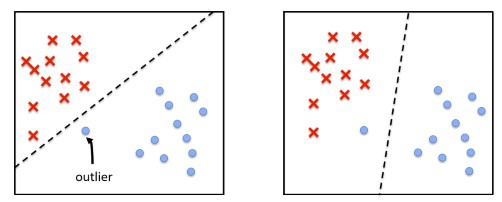
\includegraphics[scale = 1.7]{img/outliers.jpg}
        \caption{SVM in presence of outliers}
\end{figure}
The previous image shows the effect that a single outlier can have. We can make only one of the following choices: correctly classify the outlier, thus reducing the robustness of the classifier, or leave the outlier as misclassified. The strategy which is commonly adopted is the second one, as it provides more generalization to the classifier. In order to reduce the effects of mis-classification we introduce some \textbf{slack variables}, useful for allowing some errors in the boundary. More specifically, a slack variable is created for each example of the training set, and each slack variable indicates how much the constraints are violated. For example, Picture \ref{slack} shows an example of examples of the training set and the respective slack variables: in one case the value of the slack variable is 0.6, indicating that the training instance is violating the constraints of the boundary but it still classified correctly since the value is smaller than 1. In the second case, the value is 1.3, which means the instance is wrongly classified.

\begin{figure}[h!]
		\centering
		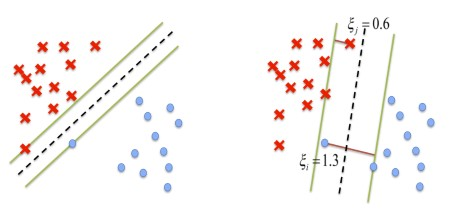
\includegraphics[scale = 1.7]{img/soft margin.jpg}
        \label{slack}
        \caption{Slack variable example}
\end{figure}

Now the optimization problem can be re-formulated as:
\begin{equation*}
\begin{aligned}
&\text{min} \quad \frac{1}{2}||w||^2+ C\sum\limits_{i = 1}^N\xi_i\\
&\text{s.t. } y_i(w^Tx_i-b)\geq 1 - \xi_i\\
&\xi_i \geq 0 \qquad i = 1,\dots,N
\end{aligned}
\end{equation*}

The only parameter C controls the \textbf{tradeoff} between the accuracy with respect to the training data and the maximization of the margin. It can be interpreted also as a \textbf{regularization term}:

\begin{itemize}
	\item small $C$ allows constraints to be easily ignored \textit{(large margin)}, allowing more misclassifications.
	\item large $C$ makes constraints hard to ignore \textit{(narrow margin)}, allowing less misclassifications.
	\item $C = \infty$ enforces all constraints \textit{(hard margin)}, so in this case no misclassification occurs.
\end{itemize}

\underline{Histograms of Oriented Gradients (HOG)}
\\

We can now focus on the method which was used to extract the feature vector from each window. The method is called \textbf{Histograms of Oriented Gradients (HOG)}, and it was introduced by \cite{dalal2005histograms}. As we said before, its goal is to create a robust feature set that allows the human form to be discriminated cleanly, even in cluttered backgrounds under difficult illumination. Picture \ref{hog} provides an overview of the feature extraction chain.

\begin{figure}[h!]
		\centering
		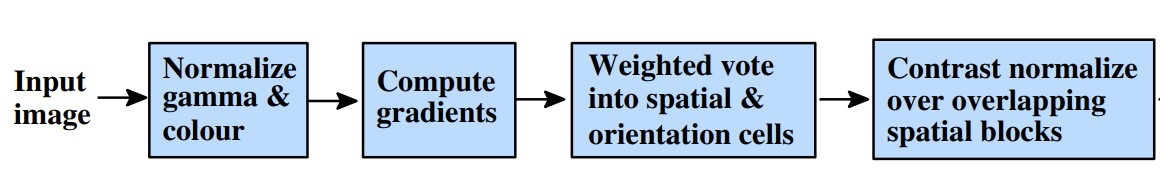
\includegraphics[scale = 1.2]{img/hog.jpg}
        \label{hog}
        \caption{Overview of HOG method}
\end{figure}

The basic idea is that local object appearance and shape can often be characterized rather well by the \textbf{distribution} of local intensity \textbf{gradients} or edge directions, even without precise knowledge of the corresponding gradient or edge positions. In this sense, we can notice that the method is based on the concept of gradient, and in particular on the distribution of gradients.

If we have a 1-variable function the gradient is computed as:

$$
\frac{df}{dx} = \lim_{\Delta x \to 0} \frac{f(x) - f(x - \Delta x)}{\Delta x} = f'(x) 
$$

Suppose that the function is discretized, i.e. it is obtained by sampling a continuous function, then the approximated gradient is given by:

$$
\frac{df}{dx} = \frac{f(x) - f(x - 1)}{1} = f(x) - f(x - 1) = f'(x) 
$$
, i.e. the approximated gradient is computed as the difference of two consecutive discrete points.

If we consider a 2-variables function, then the following relations hold:

\begin{figure}[h!]
		\centering
		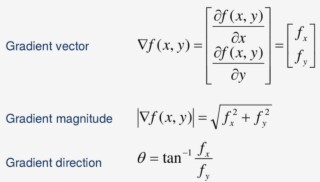
\includegraphics[scale = 1.6]{img/2dim.jpg}
\end{figure}

, so for computing each component $\frac{\delta f(x,y)}{\delta x}$ and $\frac{\delta f(x,y)}{\delta y}$ an approximation can be used. \textit{HOG} method uses the following computation:

$$
f'(x) = \lim_{h \to 0} \frac{f(x+h) - f(x-h)}{2h}
$$

Therefore, in this case if we have a point centered in $(0,0)$, then $\frac{\delta f(x,y)}{\delta x} = $ [-1, 0, 1], while $\frac{\delta f(x,y)}{\delta y} = $ \begin{bmatrix} -1 \\ 0\\ 1 \end{bmatrix}

As an example, the gradient of the pixel in Picture \ref{example} is given by $(94-56), (93-55)$, i.e. $(38, 38)^T$, while the angle is $arctan(\frac{38}{38}) = 45$ degrees.

\begin{figure}[h!]
		\centering
		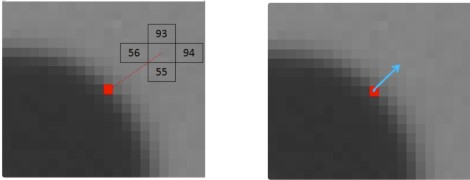
\includegraphics[scale = 1.6]{img/example.jpg}
          \label{example}
          \caption{Example of computation of the gradient and its direction}
\end{figure}

Using the gradient distribution, we can compute the gradient magnitude and direction, i.e. the angle, for each of the pixels in the image, as shown in Picture \ref{gradient_example}.

\begin{figure}[h!]
		\centering
		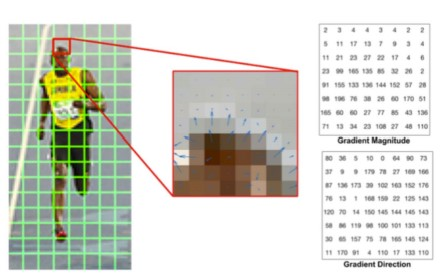
\includegraphics[scale = 2.0]{img/gradient_example.jpg}
          \label{gradient_example}
          \caption{Example of computation of the gradient and its direction for each pixel of the image}
\end{figure}

Once we introduced this method for gradient computation, we can now analyze how it is used for the task of feature extraction implemented by \textit{HOG}. This method follows these steps:

\begin{enumerate}
    \item Compute centered horizontal and vertical gradients with no smoothing;
    \item Compute gradient orientation and magnitudes (for color images, pick the color channel with the highest gradient magnitude for each pixel);
    \item Divide the 64x128 image into 16x16 blocks with 50\% of overlap (for a total of 7x15 = 105 blocks). Each block should consist of 4 cells with size 8x8, in which the gradient is computed. A visual representation of the blocks and the cells is provided in Picture \ref{cells_blocks}.

    \begin{figure}[h!]
		\centering
		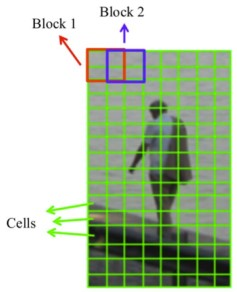
\includegraphics[scale = 2.0]{img/cells_blocks.jpg}
          \label{cells_blocks}
          \caption{Partition of the image into cells and blocks}
    \end{figure}

    \item For each 8x8 cell, compute the histogram of the gradient orientation binned into 9 bins: the vote of the cell is given by the gradient magnitude, and each vote is linearly interpolated between neighboring bin centers. For example, if the orientation is 85 degrees, then the distances to the bin center 70 and 90 are 15 and 5 degrees respectively. Hence, the vote is splitted into $\frac{5}{20} = 0.25$ for Bin 70, and $\frac{15}{20} = 0.75$ for Bin 90.

    \begin{figure}[h!]
		\centering
		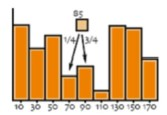
\includegraphics[scale = 2.0]{img/vote}
    \end{figure}

    Note that the vote could be also weighted with a Gaussian function in order to downweight the pixels near the edges of the block.

    \item Concatenate the 4 cell histograms in each block into a single block feature $f$ and normalize $f$ by its Euclidean norm, i.e.:

    $$
    f = \frac{f}{\sqrt{||f||_2^2 + \epsilon^2}}
    $$
    , where $\epsilon$ is used to have better performances.

    \item Finally, the final feature vector is composed of 3,780 histograms.
    
\end{enumerate}

\subsubsection{Classification phase} 
Once the feature extraction phase is done, the classification can be performed. This classification phase was composed by:

\begin{itemize}
    \item a \textbf{learning phase}, in which an SVM classifier was trained with the feature vectors resulted by the HOG method;
    \item a \textbf{test phase}, in which the classifier was asked to predict the presence or the absence of a person in each window in the image.
\end{itemize}

Since this new approach gave near-perfect separation on the original MIT pedestrian database (507 positive windows only training set, 200 positive windows only test set), the authors introduced a more challenging dataset containing over 1,800 annotated human images with a large range of pose variations and backgrounds. The training dataset was composed of 1,208 positive windows examples and 1,218 negative windows examples, generated using the \textit{Bootstrapping} technique, while the test set by 566 positive examples and 453 negative examples.

\subsubsection{Post-processing phase}
As we saw for Viola and Jones, the algorithm resulted in multiple responses around positive examples, so the \textit{non-maximum suppression} technique was performed, in order to remove all the boxes that overlapped more that 50\% with another box.

\begin{figure}[h!]
		\centering
		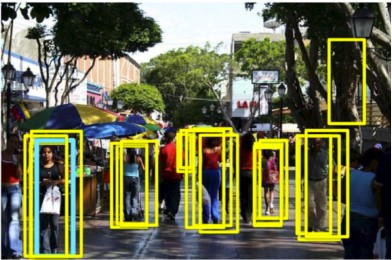
\includegraphics[scale = 2.0]{img/multiple boxes.jpg}
\end{figure}


\begin{figure}[h!]
		\centering
		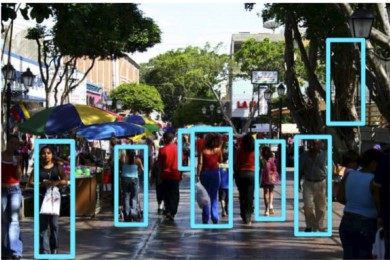
\includegraphics[scale = 2.0]{img/results.jpg}
\end{figure}
